%------------------------------------------------- 
\subsection{Discovery Strategy}
\label{subsec:fit_bh}

Model-independent fits for the discovery region are performed using \textit{pyBumpHunter} \cite{bumphunt}.
The strategy consists of comparing the data in a given \mt~spectrum of interest to a background estimation derived by performing the polynomial fit and sampling from the post-fit function into a histogram.

The polynomial fit is done to an \mt~distribution with 180 bins (25 GeV wide), half the width of the fits in the SVJ Fit region (50 GeV wide). %90 bins, as with the PFN 
The narrower bins allow for rebinning based on the \textit{signal mass resolution} of the SVJ signals.
The binning strategy is outlined in Appendix~\ref{app:binning}.

Figure~\ref{fig:bkgfit_data_crvr_antelope} shows the fit and residuals with of the polynomial with the narrower binning in the CR and the Discovery VR data.
Figure~\ref{fig:postfit_param_antelope} shows the post-fit values of the fit parameters and their uncertainties for the CR and VR. 
These results indicate good ability of the 5-parameter polynomial to model the ANTELOPE selected data.

\begin{figure}[!htbp]
\centering
   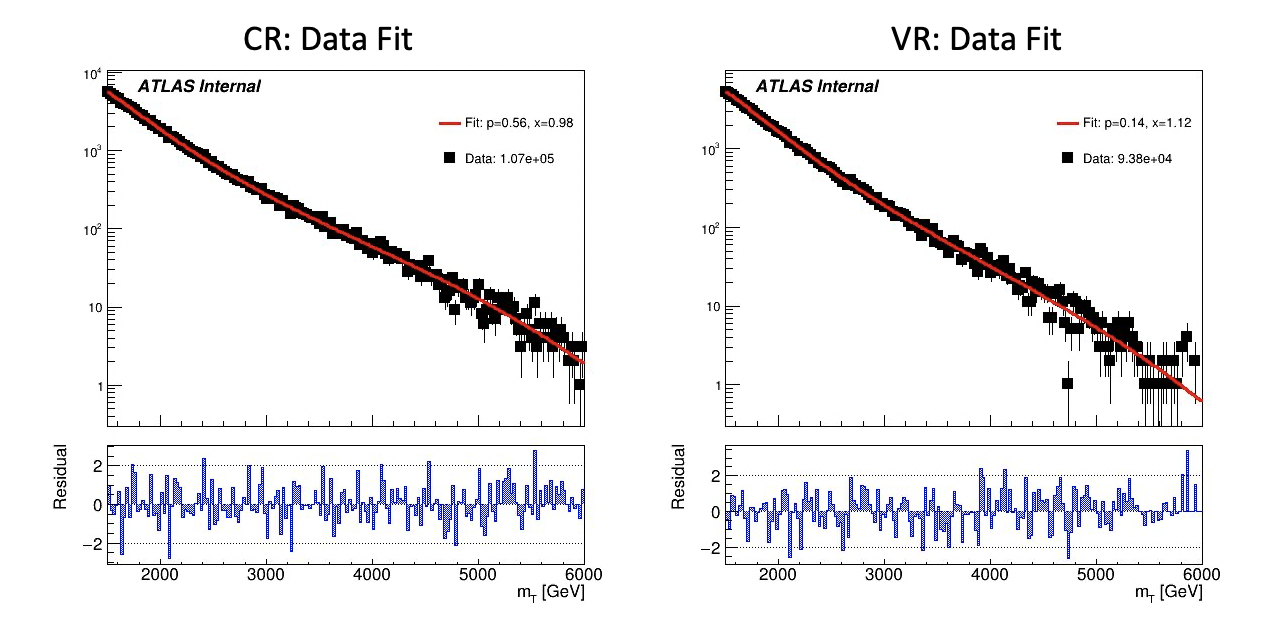
\includegraphics[width=0.95\textwidth]{figures/stats/bkgfit_data_crvr_antelope}
    \caption{Post-fit function and residuals for the ANTELOPE CR and VR.
    \label{fig:bkgfit_data_crvr_antelope}}
\end{figure}

\begin{figure}[!htbp]
\centering
   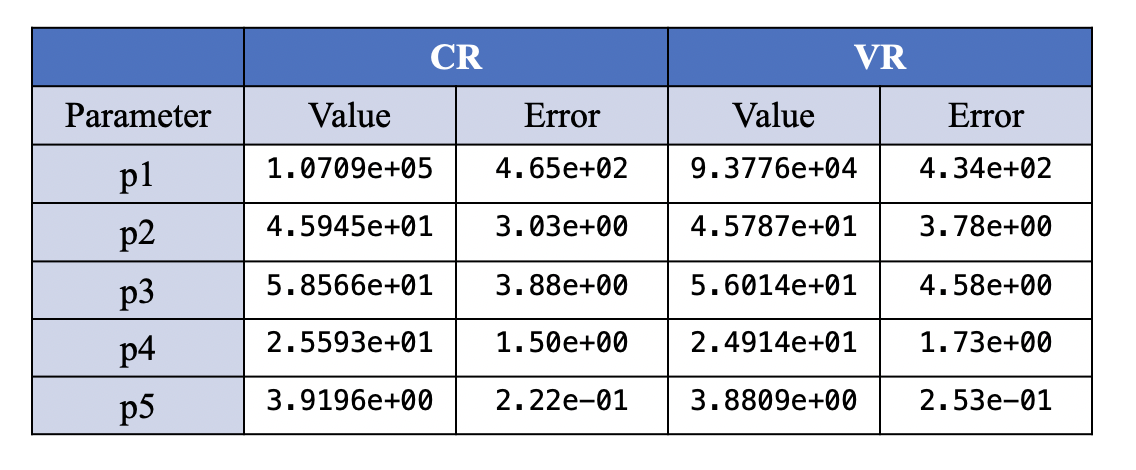
\includegraphics[width=0.65\textwidth]{figures/stats/postfit_param_antelope}
    \caption{Post-fit parameters for the ANTELOPE CR and VR.
    \label{fig:postfit_param_antelope}}
\end{figure}

The studies shown in Section~\ref{subsec:fit_bkgonly} validate the robustness of the background polynomial fit. 
The narrower bins are the only difference for polynomial fitting between the SVJ Fit and Discovery Fit strategies, and they are not observed to reduce the quality or consistency of the fit. 

%----------------------------------------------------------------------------------------
\subsubsection{BumpHunter Fits}
\label{subsec:bhfits}

The signal mass resolution binning strategy described in Appendix~\ref{app:binning} creates a monotonically increasing set of bins. 
While the SVJ signals help inform the binning, the binning is still broadly applicable to a variety of potential signal models.
The mass resolution of any resonant signal generally widens as the mass of the mediator particle increases.
A similar strategy and binning was used in the generic heavy resonance search presented in Ref.~\cite{yxh}.
The resulting set of 15 bins to be used in the BumpHunter fits varies in width from 100 GeV at the \mt~core to 925 GV in the \mt~tail. 

Figure~\ref{fig:antelope_bh_crvr} shows the result of running BumpHunter over the rebinned CR and VR \mt~spectra.
The background estimation is given by polynomial fit function. 
The high p-values (>0.01) indicate good agreement with the background estimation.
\begin{figure}[!htbp]
\centering
   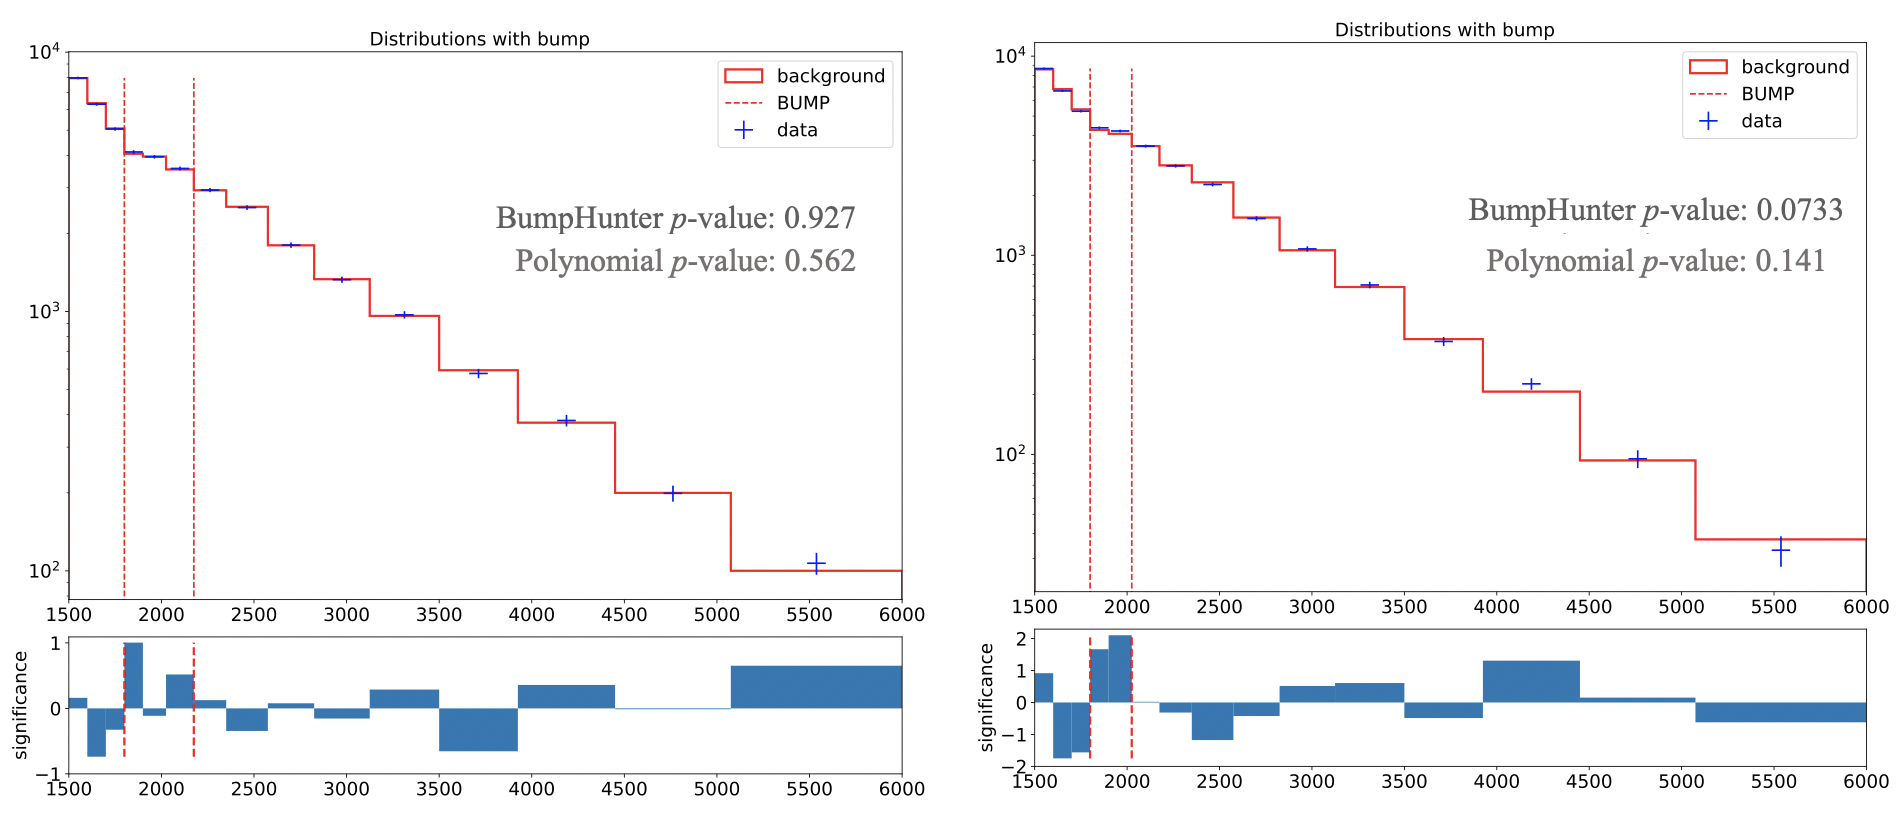
\includegraphics[width=0.95\textwidth]{figures/stats/antelope_bh_crvr}
    \caption{BumpHunter fits on the ANTELOPE \mt~spectra for both the CR (left) and VR (right). In a signal-depleted region, good agreement with the background estimation is observed.
    \label{fig:antelope_bh_crvr}}
\end{figure}

Figure~\ref{fig:bh_asimov_pvals} shows BumpHunter p-values over 100 Asimov trials, where each toy is scaled to the statistics of the SR.
The agreement is generally very good, as the p-values trend towards higher values.
No fits with a \textit{spurious signal} are found.
A spurious signal would be indicated by a fit with a p-value $<$ 0.01, indicting a bump of at least $2\sigma$ significance.
\begin{figure}[!htbp]
\centering
   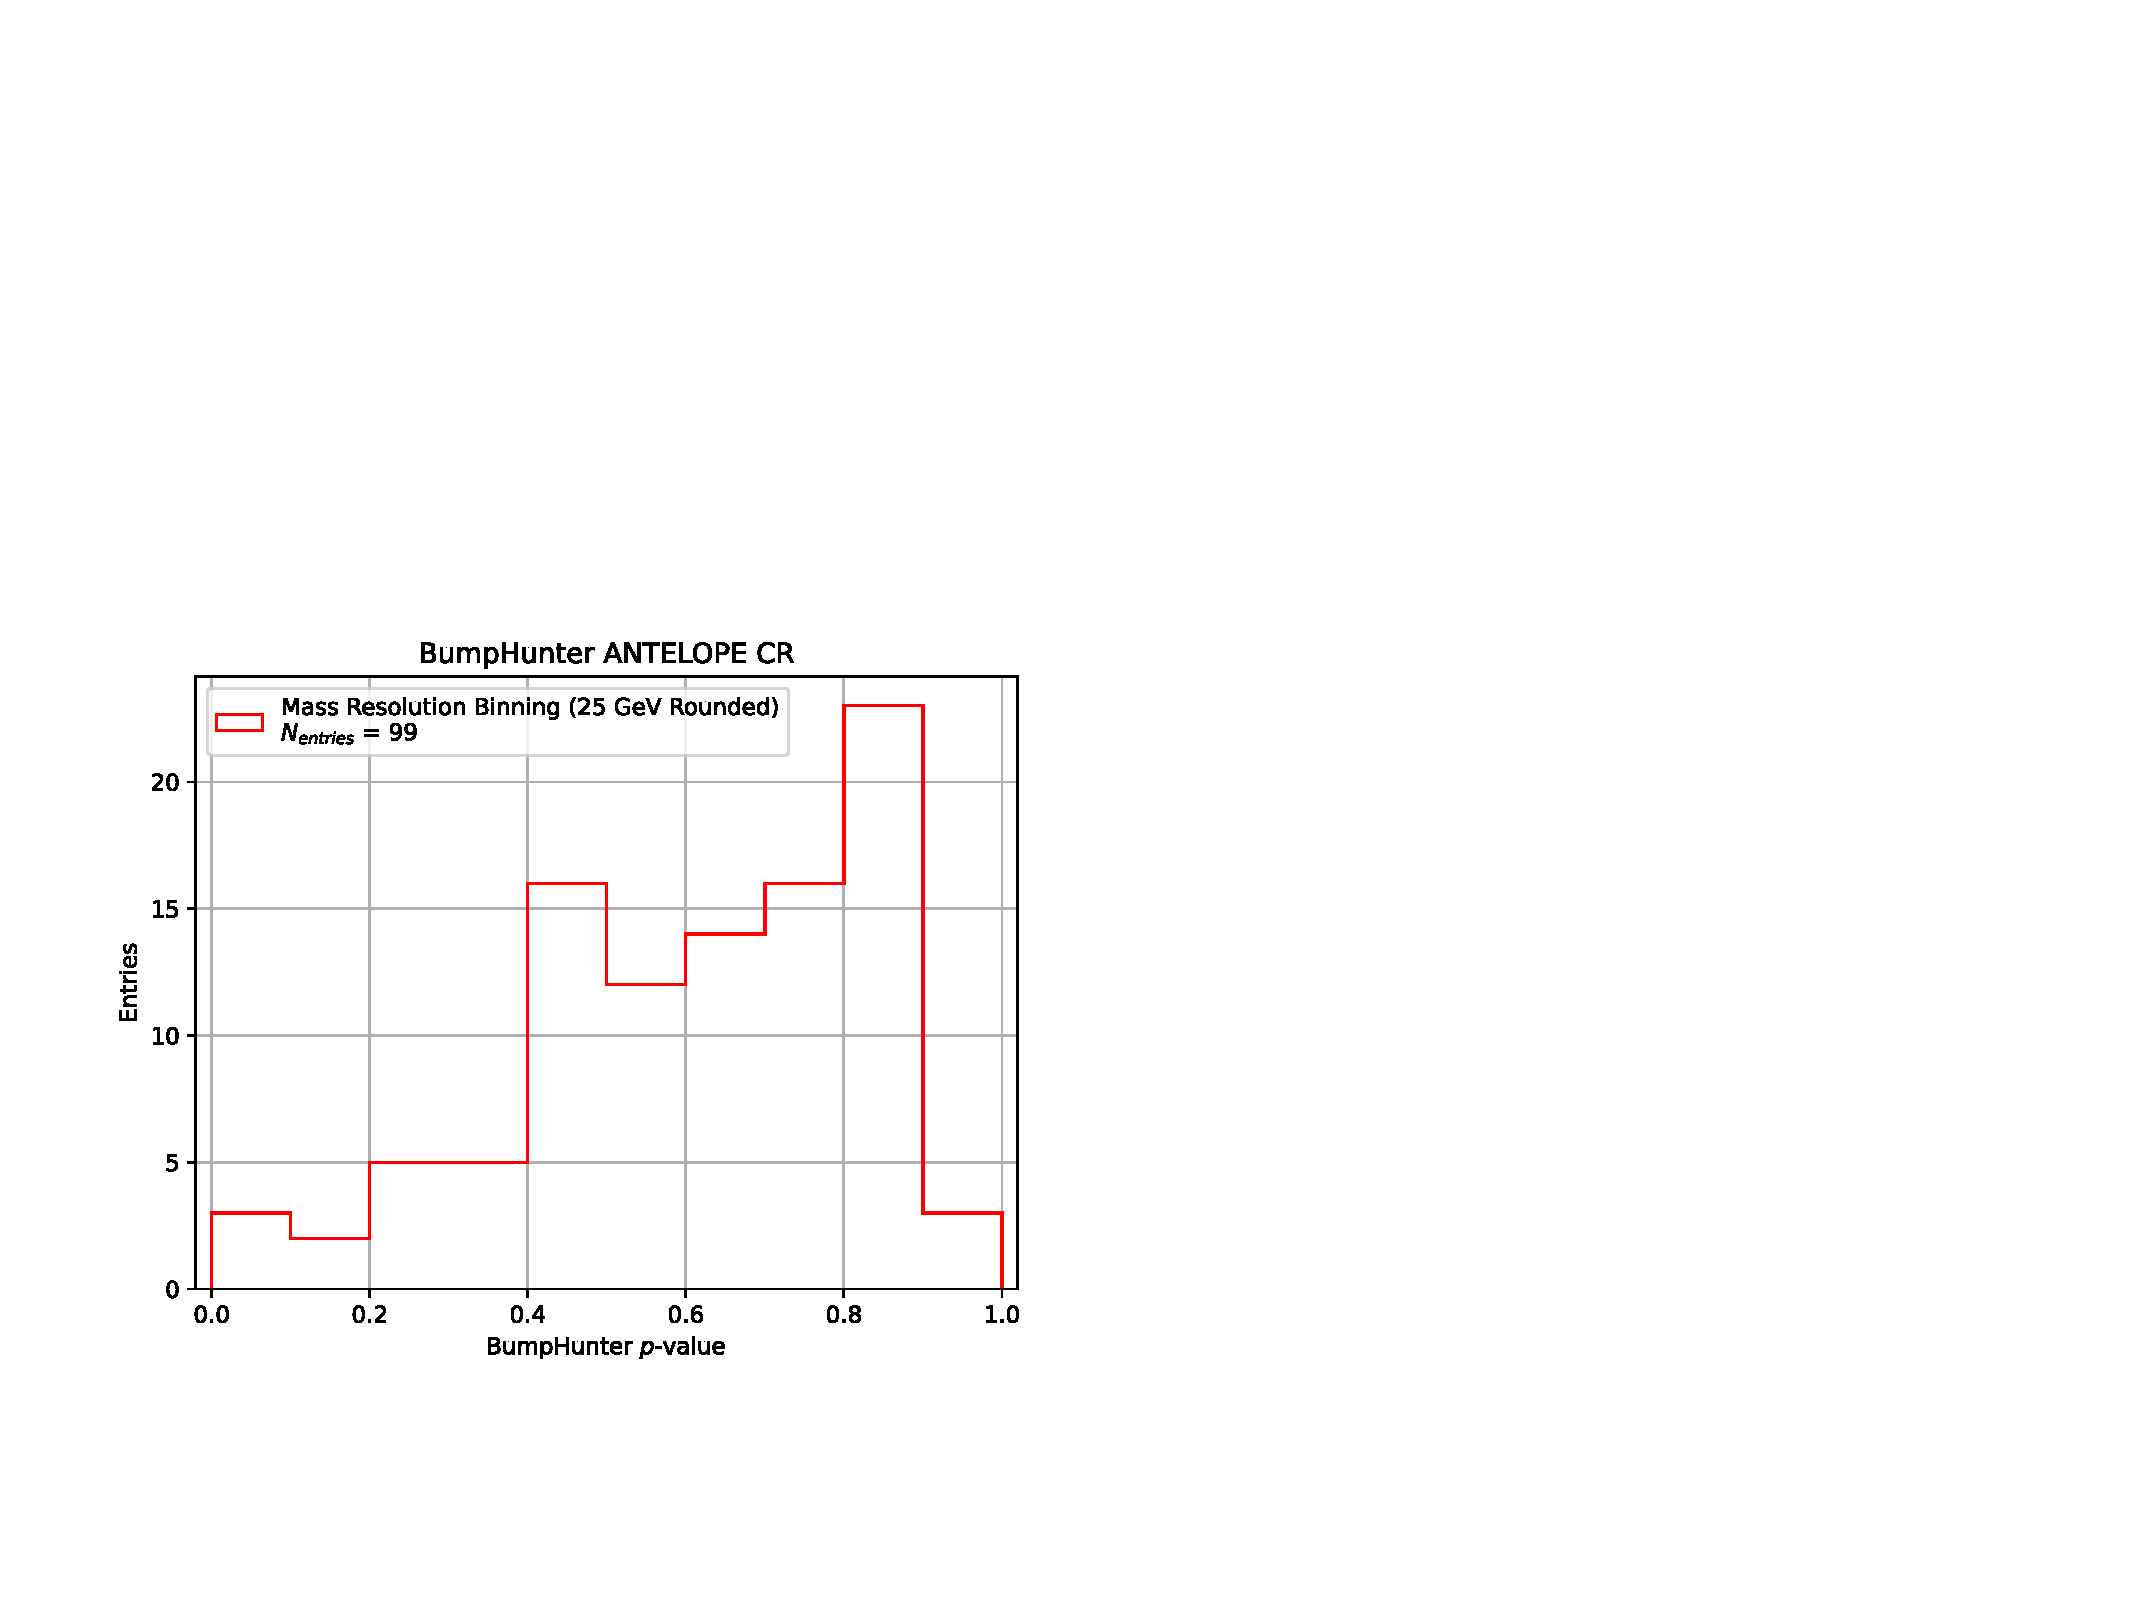
\includegraphics[width=0.45\textwidth]{figures/stats/bh_asimov_pvals_cr}
   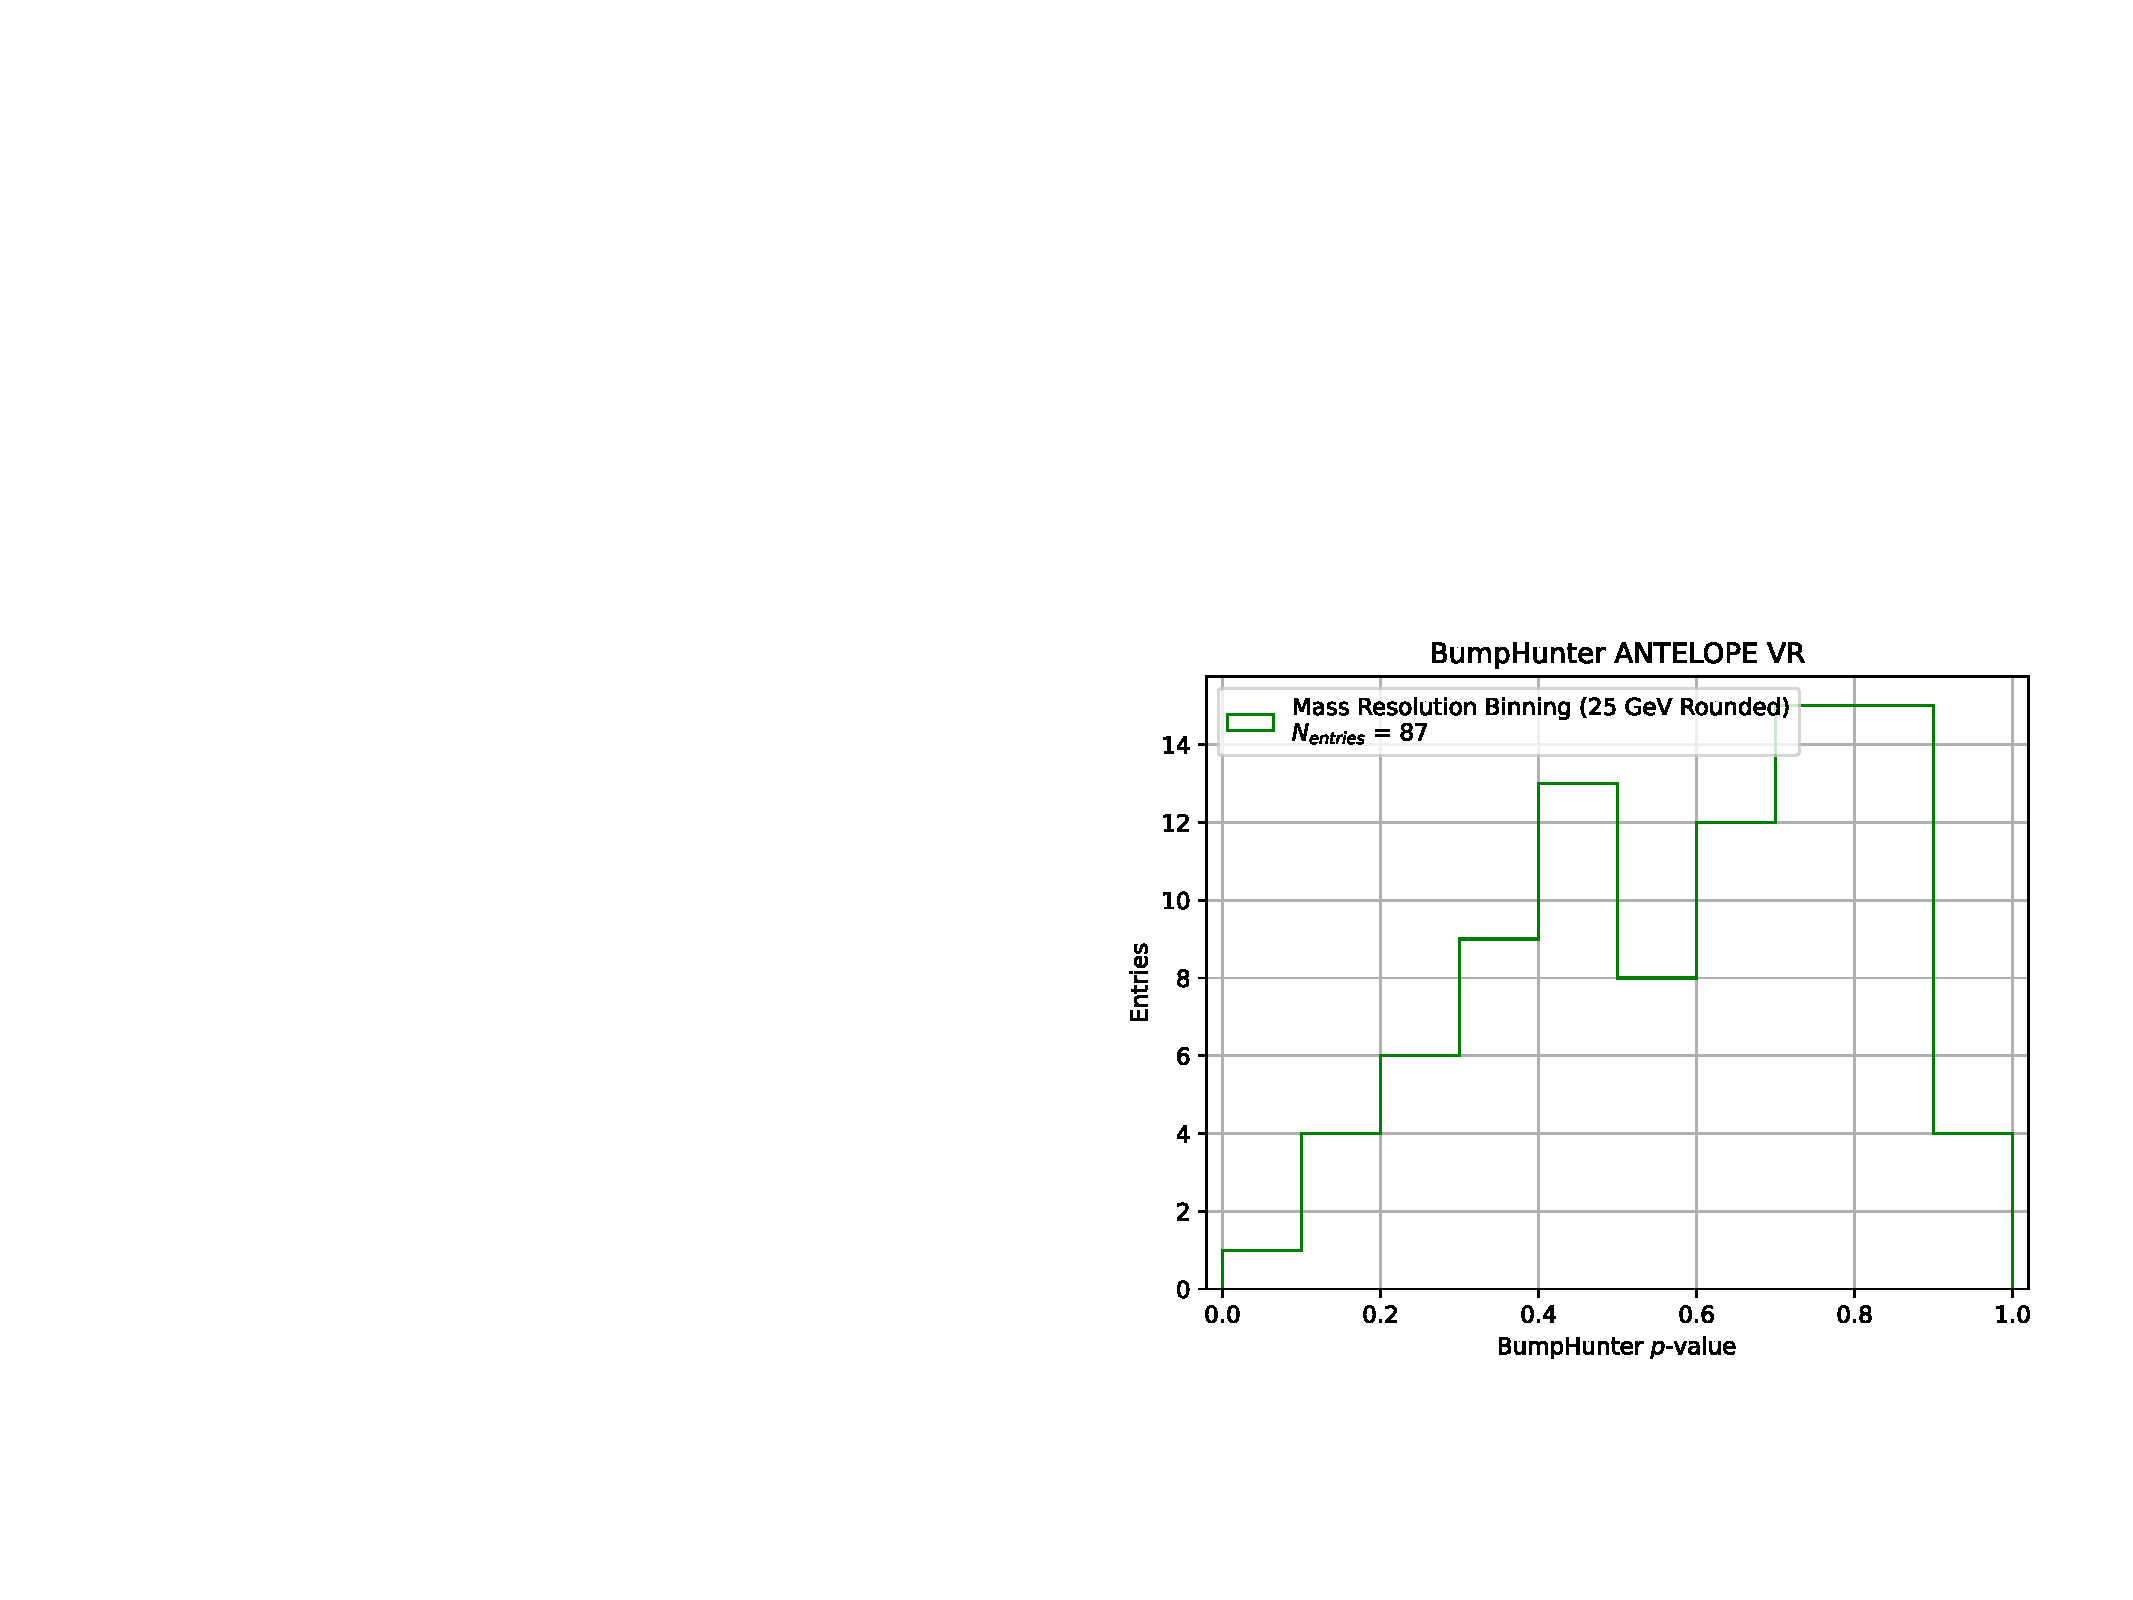
\includegraphics[width=0.45\textwidth]{figures/stats/bh_asimov_pvals_vr}
    \caption{BumpHunter p-values extracted for 100 Asimov toys for both the ANTELOPE CR (left) and VR (right).
    \label{fig:bh_asimov_pvals}}
\end{figure}




